\begin{figure}[H]
    \centering
    \foreach \i in {1,..., 7}{
    \begin{subfigure}{\textwidth}
% include second image
        \includegraphics[width=\textwidth]{images/latent_space_traversals/vae_dsprites_7500_rotation_\i.png}
    \end{subfigure}}
    \caption[7,500-VAE - Rotation traversal]{Latent spaces traversal between different rotation values for 7,500-\ac{VAE} on the dSprites dataset}
    \label{fig:vae_dsprites_rotation_vae_7500}
\end{figure}

\begin{figure}[H]
    \centering
    \foreach \i in {1,..., 7}{
    \begin{subfigure}{\textwidth}
% include second image
        \includegraphics[width=\textwidth]{images/latent_space_traversals/vae_dsprites_lf_6250_rotation_\i.png}
    \end{subfigure}}
    \caption[6,250-VAE - Rotation traversal]{Latent spaces traversal between different rotation values for 6,250-\ac{VAE} on the dSprites dataset}
    \label{fig:vae_dsprites_rotation_vae_6250}
\end{figure}

\begin{figure}[H]
    \centering
    \foreach \i in {1,..., 7}{
    \begin{subfigure}{\textwidth}
% include second image
        \includegraphics[width=\textwidth]{images/latent_space_traversals/vae_dsprites_5000_rotation_\i.png}
    \end{subfigure}}
    \caption[5,000-VAE - Rotation traversal]{Latent spaces traversal between different rotation values for 5,000-\ac{VAE} on the dsprites dataset}
    \label{fig:vae_dsprites_rotation_vae_5000}
\end{figure}

\begin{figure}[H]
    \centering
    \foreach \i in {1,..., 7}{
    \begin{subfigure}{\textwidth}
% include second image
        \includegraphics[width=\textwidth]{images/latent_space_traversals/vae_dsprites_3750_rotation_\i.png}
    \end{subfigure}}
    \caption[3,750-VAE - Rotation traversal]{Latent spaces traversal between different rotation values for 3,750-\ac{VAE} on the dsprites dataset}
    \label{fig:vae_dsprites_rotation_vae_3750}
\end{figure}

\begin{figure}[H]
    \centering
    \begin{subfigure}{.48\textwidth}
% include second image
        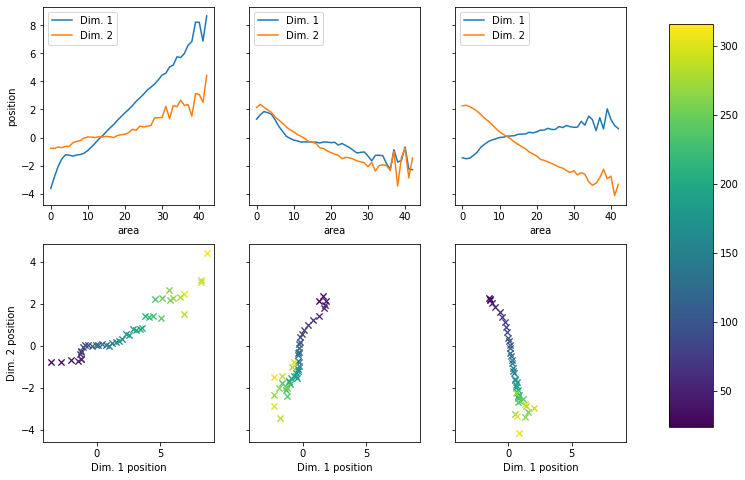
\includegraphics[width=\textwidth]{images/latent_space_traversals/vlae_gan_mnist_morpho_latent_space_values_area.png}
        \caption{area}
    \end{subfigure}
    \hfill
    \begin{subfigure}{.48\textwidth}
% include second image
        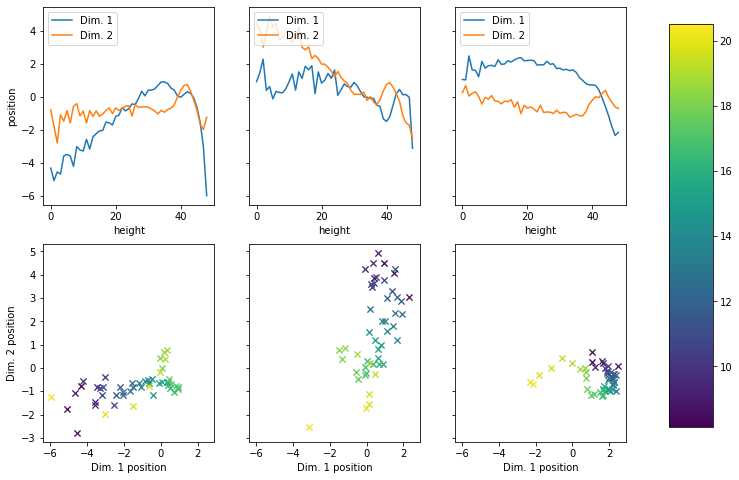
\includegraphics[width=\textwidth]{images/latent_space_traversals/vlae_gan_mnist_morpho_latent_space_values_height.png}
        \caption{height}
    \end{subfigure}
    \begin{subfigure}{.48\textwidth}
% include second image
        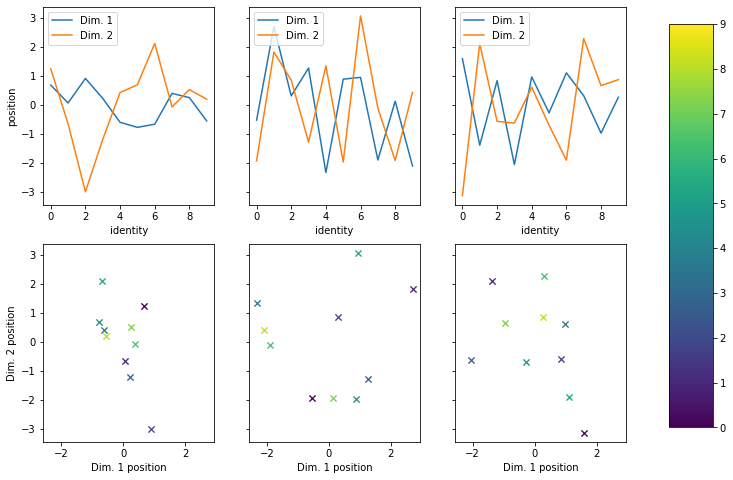
\includegraphics[width=\textwidth]{images/latent_space_traversals/vlae_gan_mnist_morpho_latent_space_values_identity.png}
        \caption{identity}
    \end{subfigure}
    \hfill
    \begin{subfigure}{.48\textwidth}
% include second image
        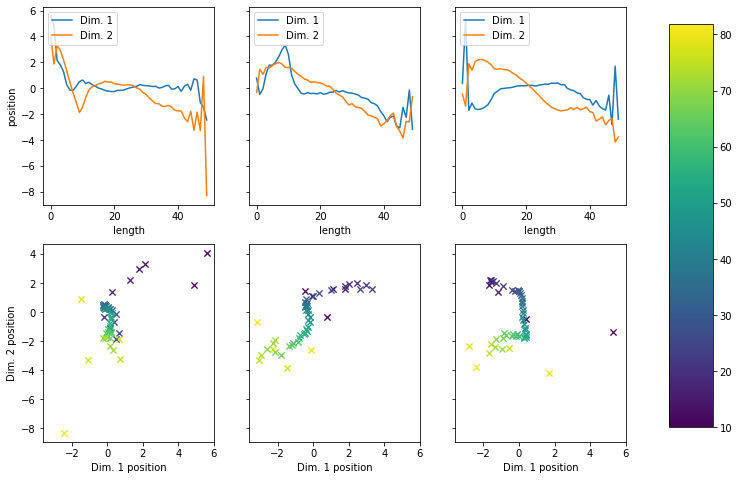
\includegraphics[width=\textwidth]{images/latent_space_traversals/vlae_gan_mnist_morpho_latent_space_values_length.png}
        \caption{length}
    \end{subfigure}
    \begin{subfigure}{.48\textwidth}
% include second image
        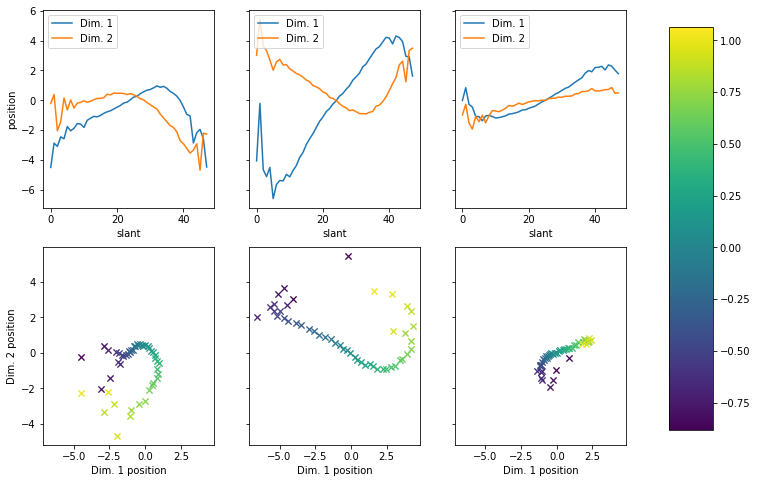
\includegraphics[width=\textwidth]{images/latent_space_traversals/vlae_gan_mnist_morpho_latent_space_values_slant.png}
        \caption{slant}
    \end{subfigure}
    \hfill
    \begin{subfigure}{.48\textwidth}
% include second image
        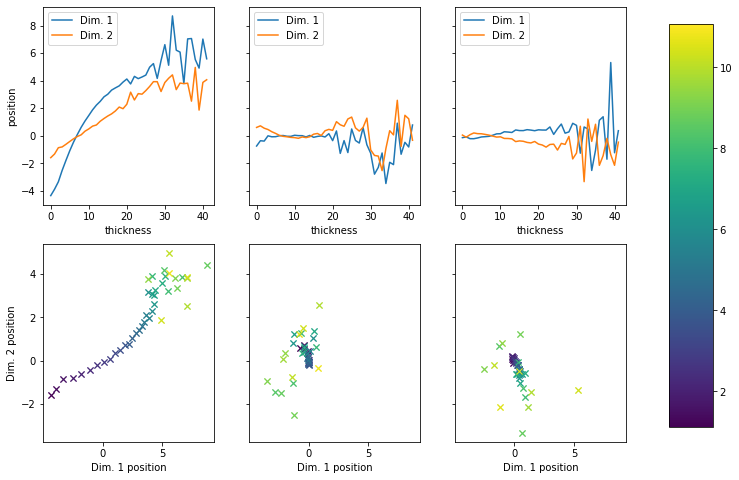
\includegraphics[width=\textwidth]{images/latent_space_traversals/vlae_gan_mnist_morpho_latent_space_values_thickness.png}
        \caption{thickness}
    \end{subfigure}
    \begin{subfigure}{.48\textwidth}
% include second image
        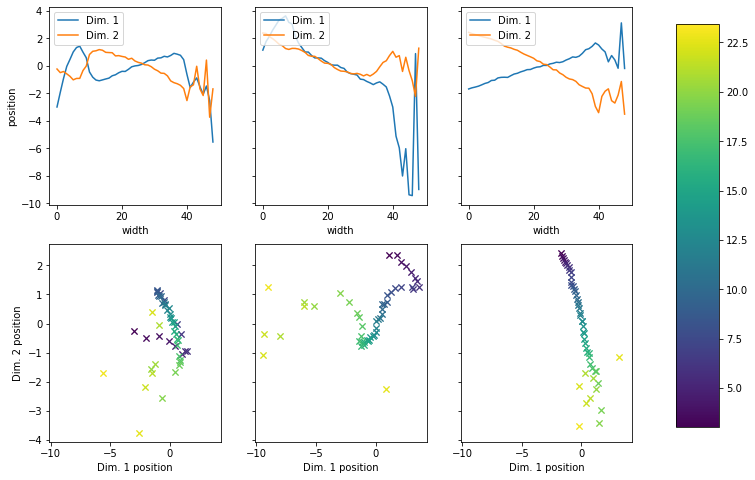
\includegraphics[width=\textwidth]{images/latent_space_traversals/vlae_gan_mnist_morpho_latent_space_values_width.png}
        \caption{width}
    \end{subfigure}
    \caption[\textsc{Mnist}-VLAE-GAN - Latent Space Values]{Mean latent space values for \textsc{Mnist}-VLAE-GAN when fixing different factors of variation from Morpho-\textsc{Mnist}}
    \label{fig:appendix_vlae_gan_mnist_latent_space_morpho}

\end{figure}

\begin{figure}[H]
    \centering
    \begin{subfigure}{.48\textwidth}
% include second image
        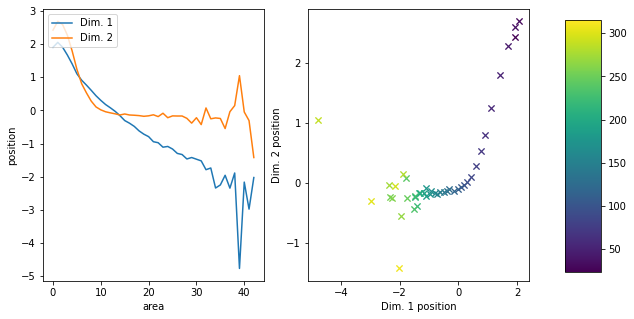
\includegraphics[width=\textwidth]{images/latent_space_traversals/vae_mnist_morpho_latent_space_values_area.png}
        \caption{area}
    \end{subfigure}
    \hfill
    \begin{subfigure}{.48\textwidth}
% include second image
        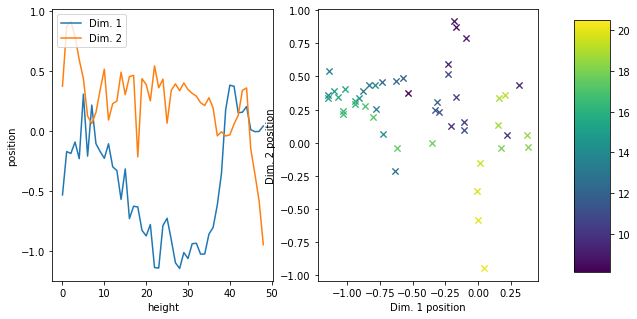
\includegraphics[width=\textwidth]{images/latent_space_traversals/vae_mnist_morpho_latent_space_values_height.png}
        \caption{height}
    \end{subfigure}
    \begin{subfigure}{.48\textwidth}
% include second image
        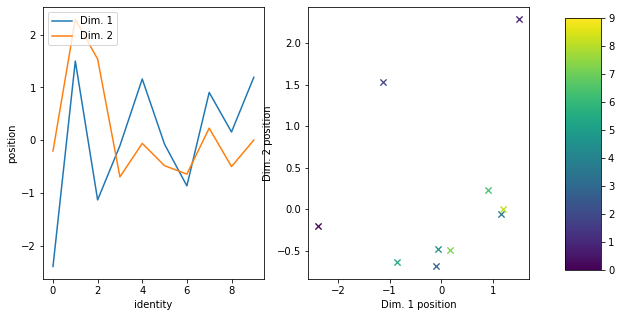
\includegraphics[width=\textwidth]{images/latent_space_traversals/vae_mnist_morpho_latent_space_values_identity.png}
        \caption{identity}
    \end{subfigure}
    \hfill
    \begin{subfigure}{.48\textwidth}
% include second image
        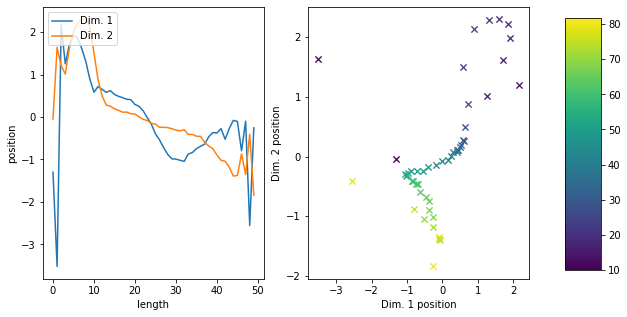
\includegraphics[width=\textwidth]{images/latent_space_traversals/vae_mnist_morpho_latent_space_values_length.png}
        \caption{length}
    \end{subfigure}
    \begin{subfigure}{.48\textwidth}
% include second image
        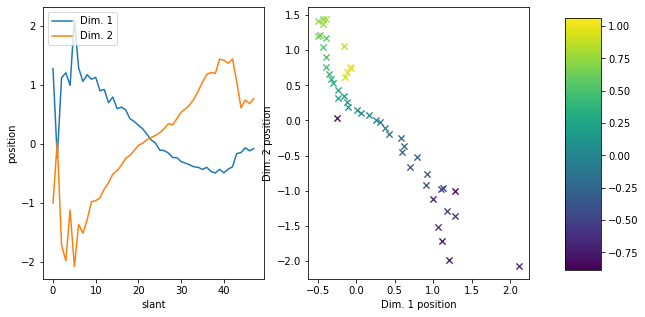
\includegraphics[width=\textwidth]{images/latent_space_traversals/vae_mnist_morpho_latent_space_values_slant.png}
        \caption{slant}
    \end{subfigure}
    \hfill
    \begin{subfigure}{.48\textwidth}
% include second image
        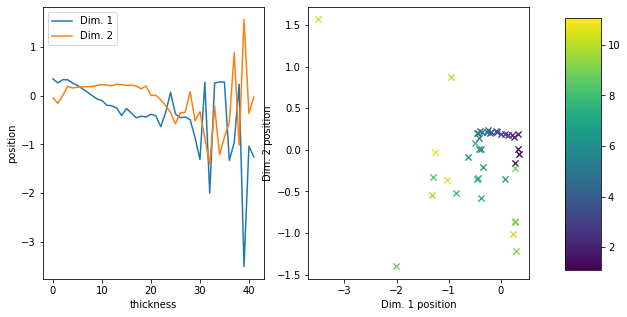
\includegraphics[width=\textwidth]{images/latent_space_traversals/vae_mnist_morpho_latent_space_values_thickness.png}
        \caption{thickness}
    \end{subfigure}
    \begin{subfigure}{.48\textwidth}
% include second image
        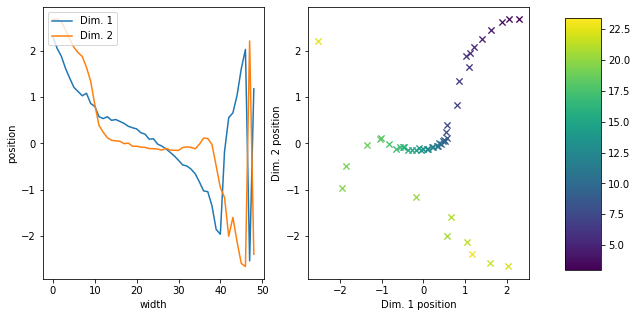
\includegraphics[width=\textwidth]{images/latent_space_traversals/vae_mnist_morpho_latent_space_values_width.png}
        \caption{width}
    \end{subfigure}
    \caption[\textsc{Mnist}-VAE - Latent Space Values]{Mean latent space values for \textsc{Mnist}-VAE when fixing different factors of variation from Morpho-\textsc{Mnist}}
    \label{fig:vae_mnist_morpho_latent_space_values}
\end{figure}

\begin{figure}[H]
    \centering
    \begin{subfigure}{.48\textwidth}
% include second image
        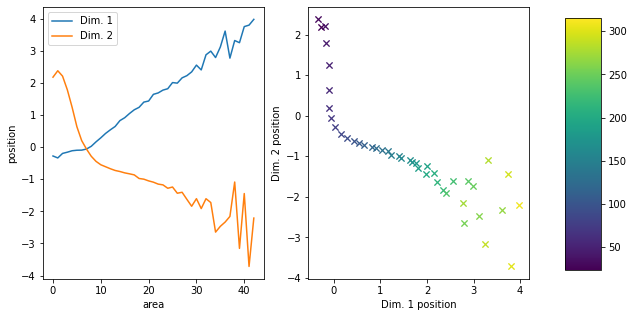
\includegraphics[width=\textwidth]{images/latent_space_traversals/vae_gan_mnist_morpho_latent_space_values_area.png}
        \caption{area}
    \end{subfigure}
    \hfill
    \begin{subfigure}{.48\textwidth}
% include second image
        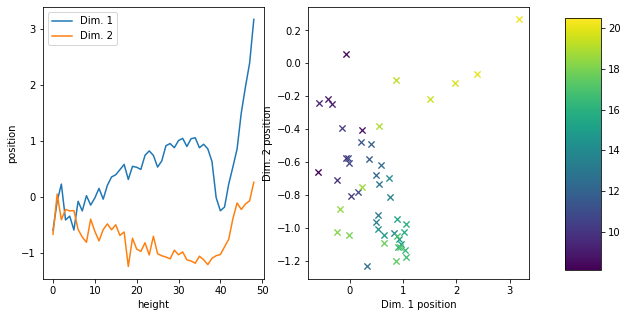
\includegraphics[width=\textwidth]{images/latent_space_traversals/vae_gan_mnist_morpho_latent_space_values_height.png}
        \caption{height}
    \end{subfigure}
    \begin{subfigure}{.48\textwidth}
% include second image
        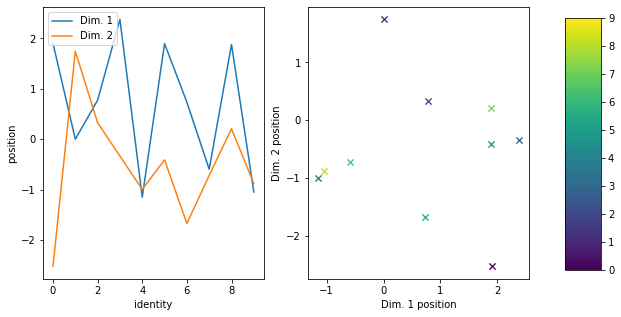
\includegraphics[width=\textwidth]{images/latent_space_traversals/vae_gan_mnist_morpho_latent_space_values_identity.png}
        \caption{identity}
    \end{subfigure}
    \hfill
    \begin{subfigure}{.48\textwidth}
% include second image
        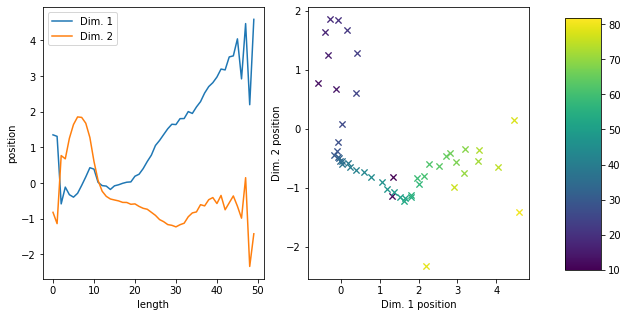
\includegraphics[width=\textwidth]{images/latent_space_traversals/vae_gan_mnist_morpho_latent_space_values_length.png}
        \caption{length}
    \end{subfigure}
    \begin{subfigure}{.48\textwidth}
% include second image
        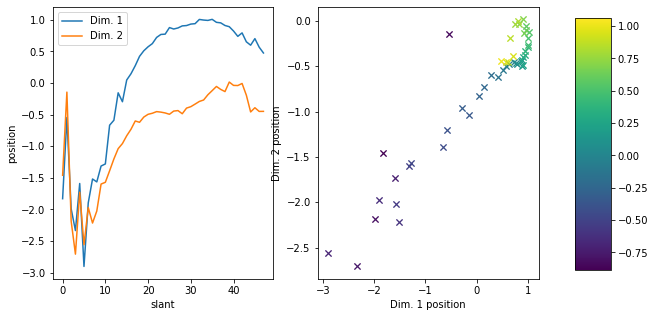
\includegraphics[width=\textwidth]{images/latent_space_traversals/vae_gan_mnist_morpho_latent_space_values_slant.png}
        \caption{slant}
    \end{subfigure}
    \hfill
    \begin{subfigure}{.48\textwidth}
% include second image
        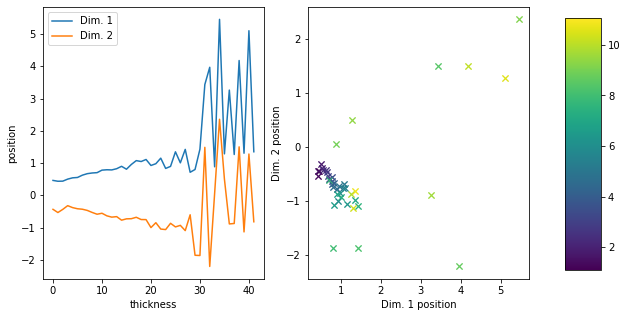
\includegraphics[width=\textwidth]{images/latent_space_traversals/vae_gan_mnist_morpho_latent_space_values_thickness.png}
        \caption{thickness}
    \end{subfigure}
    \begin{subfigure}{.48\textwidth}
% include second image
        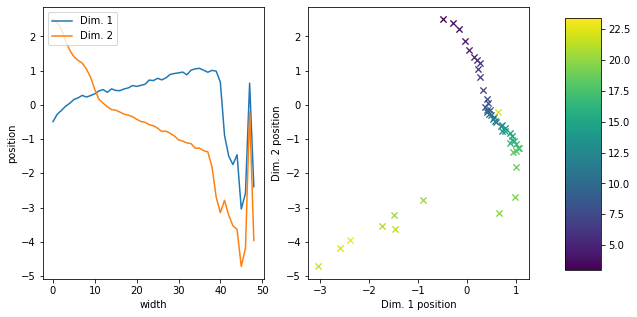
\includegraphics[width=\textwidth]{images/latent_space_traversals/vae_gan_mnist_morpho_latent_space_values_width.png}
        \caption{width}
    \end{subfigure}
    \caption[\textsc{Mnist}-VAE-GAN - Latent Space Values]{Mean latent space values for \textsc{Mnist}-VAE-GAN when fixing different factors of variation from Morpho-\textsc{Mnist}}
    \label{fig:vae_gan_mnist_morpho_latent_space_values}
\end{figure}

\begin{figure}[H]
    \centering
    \begin{subfigure}{.48\textwidth}
% include second image
        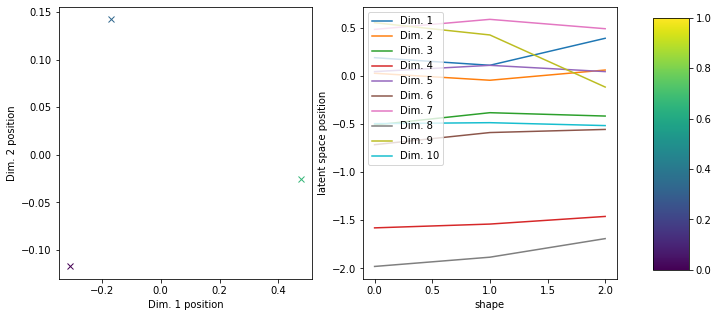
\includegraphics[width=\textwidth]{images/latent_space_traversals/vae_10000_dsprites_latent_space_values_shape.png}
        \caption{Traversal of the reduced latent space for different shapes.}
    \end{subfigure}
    \begin{subfigure}{.48\textwidth}
% include second image
        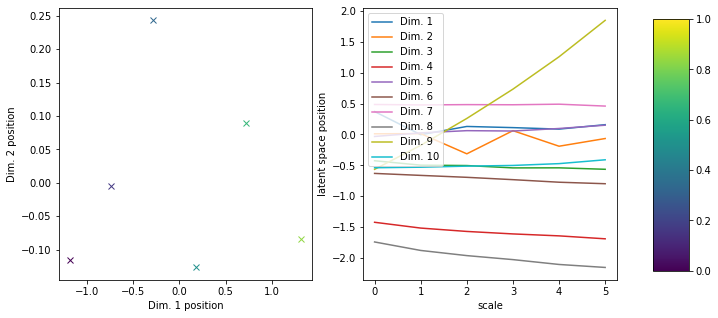
\includegraphics[width=\textwidth]{images/latent_space_traversals/vae_10000_dsprites_latent_space_values_scale.png}
        \caption{Traversal of the reduced latent space for different scales.}
    \end{subfigure}
    \begin{subfigure}{.48\textwidth}
% include second image
        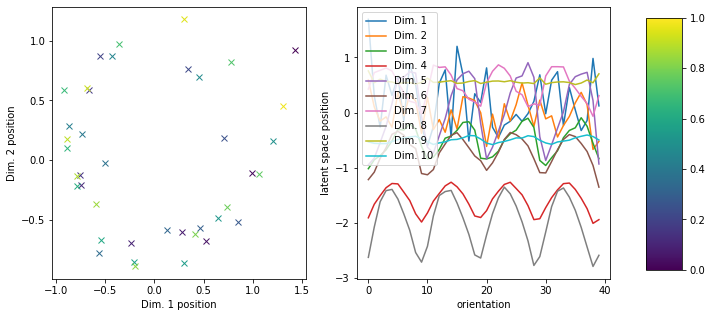
\includegraphics[width=\textwidth]{images/latent_space_traversals/vae_10000_dsprites_latent_space_values_orientation.png}
        \caption{Traversal of the reduced latent space for different orientations.}
    \end{subfigure}
    \caption[10,000-VAE - Latent Space Values]{Latent space of 10,000-\ac{VAE}. Different values are either for different $x$-positions or for different $y$-position. The other position is fixed to 1.0. It is averaged over all other parameters.}
    \label{fig:vae_dsprites_10000_latent_space_position}
\end{figure}

\begin{figure}[H]
    \centering
    \begin{subfigure}{.48\textwidth}
% include second image
        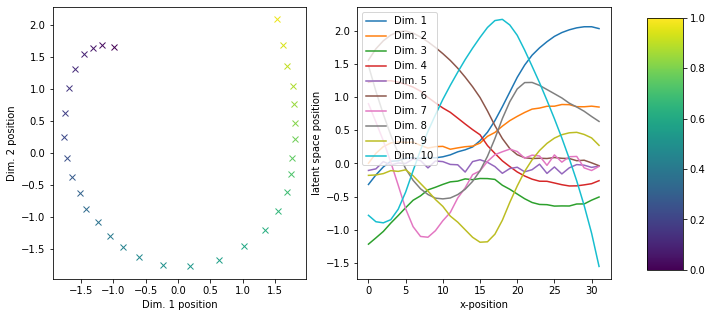
\includegraphics[width=\textwidth]{images/latent_space_traversals/vae_7500_dsprites_latent_space_values_x_position.png}
        \caption{Traversal of the reduced latent space for different $x$-positions.}
    \end{subfigure}
    \begin{subfigure}{.48\textwidth}
% include second image
        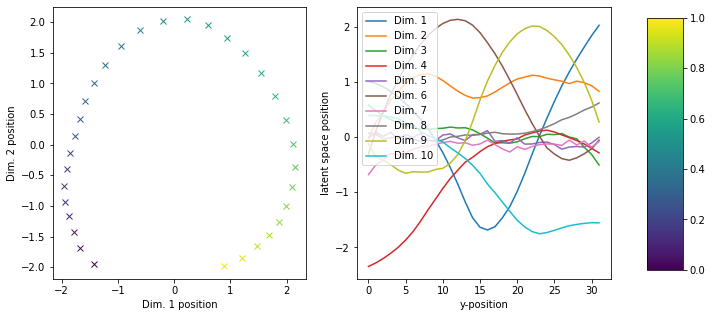
\includegraphics[width=\textwidth]{images/latent_space_traversals/vae_7500_dsprites_latent_space_values_y_position.png}
        \caption{Traversal of the reduced latent space for different $y$-positions.}
    \end{subfigure}
    \begin{subfigure}{.48\textwidth}
% include second image
        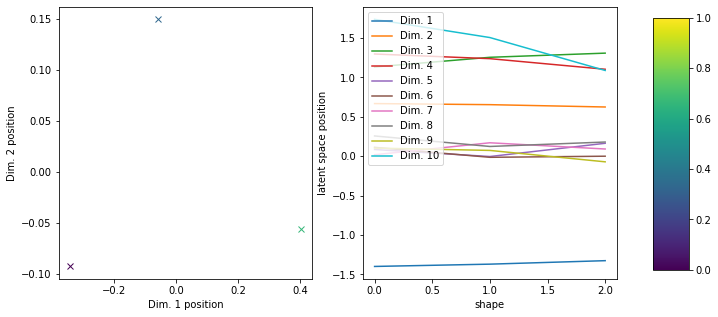
\includegraphics[width=\textwidth]{images/latent_space_traversals/vae_7500_dsprites_latent_space_values_shape.png}
        \caption{Traversal of the reduced latent space for different shapes.}
    \end{subfigure}
    \begin{subfigure}{.48\textwidth}
% include second image
        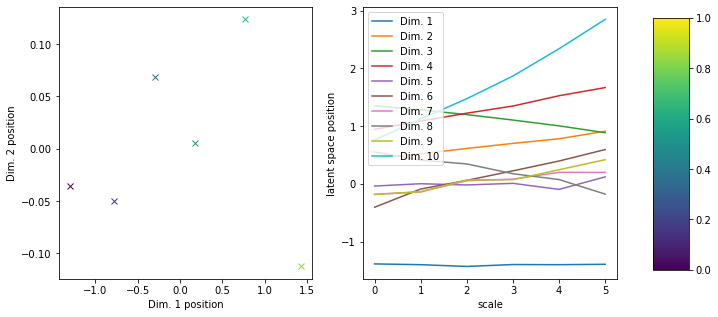
\includegraphics[width=\textwidth]{images/latent_space_traversals/vae_7500_dsprites_latent_space_values_scale.png}
        \caption{Traversal of the reduced latent space for different scales.}
    \end{subfigure}
    \begin{subfigure}{.48\textwidth}
% include second image
        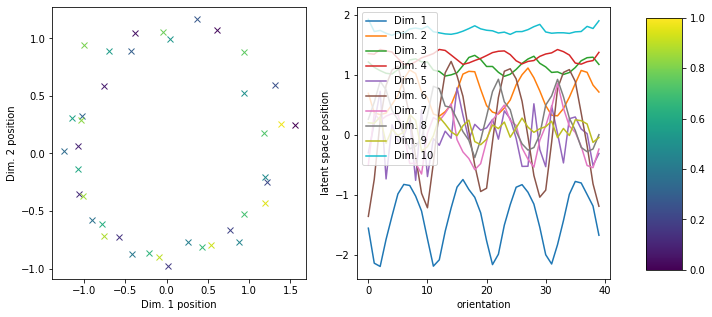
\includegraphics[width=\textwidth]{images/latent_space_traversals/vae_7500_dsprites_latent_space_values_orientation.png}
        \caption{Traversal of the reduced latent space for different orientations.}
    \end{subfigure}
    \caption[7,500-VAE - Latent Space Values]{Latent space of 7,500-\ac{VAE}. Different values are either for different $x$-positions or for different $y$-position. The other position is fixed to 1.0. It is averaged over all other parameters.}
    \label{fig:vae_dsprite_7500_latent_space_position}
\end{figure}

\begin{figure}[H]
    \centering
    \begin{subfigure}{.48\textwidth}
% include second image
        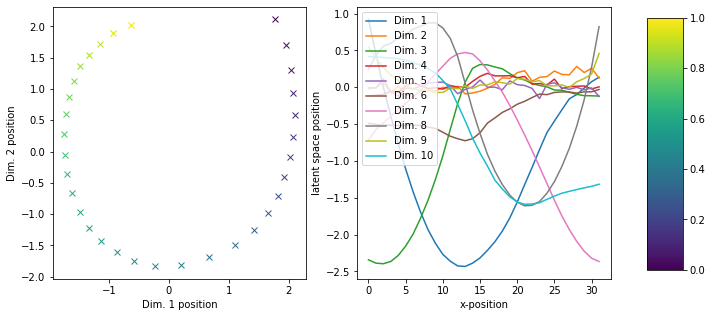
\includegraphics[width=\textwidth]{images/latent_space_traversals/vae_6250_dsprites_latent_space_values_x_position.png}
        \caption{Traversal of the reduced latent space for different $x$-positions.}
    \end{subfigure}
    \begin{subfigure}{.48\textwidth}
% include second image
        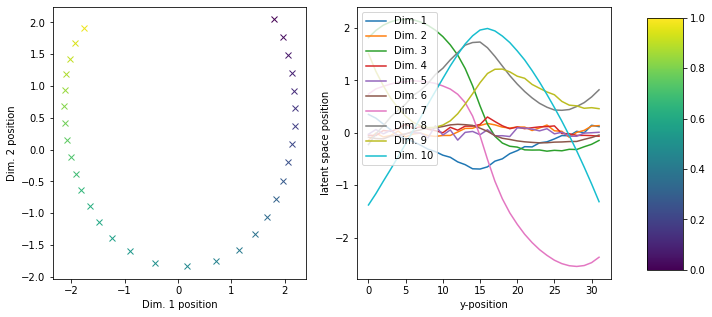
\includegraphics[width=\textwidth]{images/latent_space_traversals/vae_6250_dsprites_latent_space_values_y_position.png}
        \caption{Traversal of the reduced latent space for different $y$-positions.}
    \end{subfigure}
    \begin{subfigure}{.48\textwidth}
% include second image
        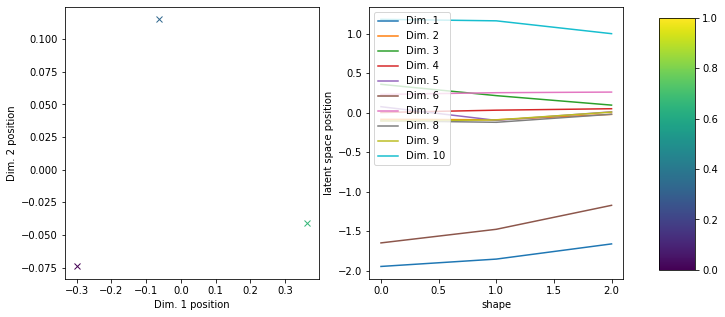
\includegraphics[width=\textwidth]{images/latent_space_traversals/vae_6250_dsprites_latent_space_values_shape.png}
        \caption{Traversal of the reduced latent space for different shapes.}
    \end{subfigure}
    \begin{subfigure}{.48\textwidth}
% include second image
        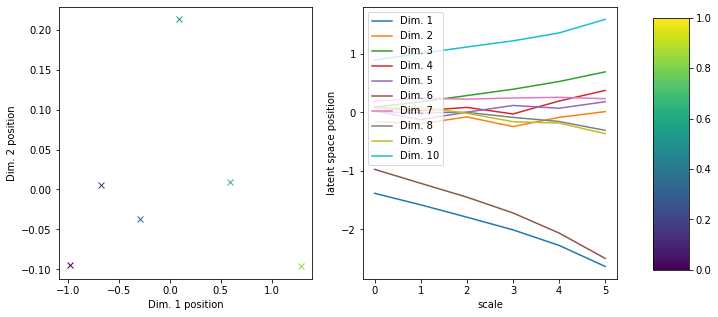
\includegraphics[width=\textwidth]{images/latent_space_traversals/vae_6250_dsprites_latent_space_values_scale.png}
        \caption{Traversal of the reduced latent space for different scales.}
    \end{subfigure}
    \begin{subfigure}{.48\textwidth}
% include second image
        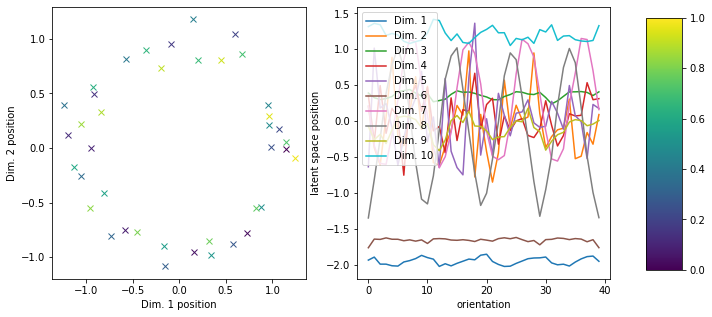
\includegraphics[width=\textwidth]{images/latent_space_traversals/vae_6250_dsprites_latent_space_values_orientation.png}
        \caption{Traversal of the reduced latent space for different orientations.}
    \end{subfigure}
    \caption[6,250-VAE - Latent Space Values]{Latent space of 6,250-\ac{VAE}. Different values correspond to different values for the respective factor of variation. For orientation and scale, the position is fixed to 0.0 in both directions, shape is fixed to \textit{Square}. For $x$-and $y$-postition, the other position is fixed to 1.0 and shape is fixed to \textit{Square}.}
    \label{fig:vae_dsprite_6250_latent_space_position}
\end{figure}

\begin{figure}[H]
    \centering
    \begin{subfigure}{.48\textwidth}
% include second image
        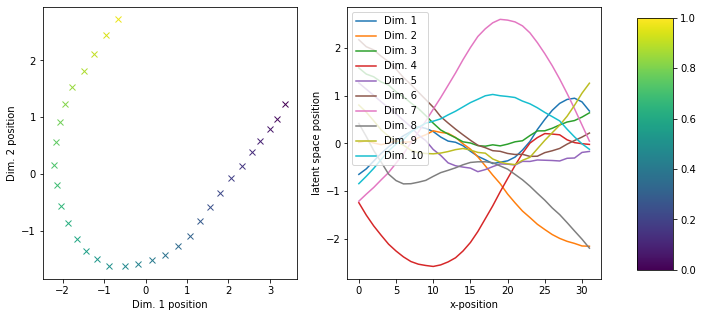
\includegraphics[width=\textwidth]{images/latent_space_traversals/vae_5000_dsprites_latent_space_values_x_position.png}
        \caption{Traversal of the reduced latent space for different $x$-positions.}
    \end{subfigure}
    \begin{subfigure}{.48\textwidth}
% include second image
        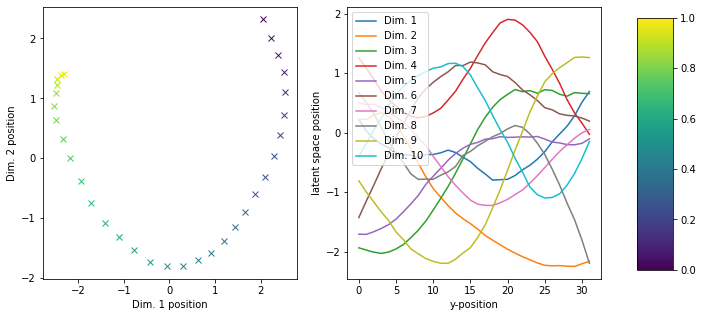
\includegraphics[width=\textwidth]{images/latent_space_traversals/vae_5000_dsprites_latent_space_values_y_position.png}
        \caption{Traversal of the reduced latent space for different $y$-positions.}
    \end{subfigure}
    \begin{subfigure}{.48\textwidth}
% include second image
        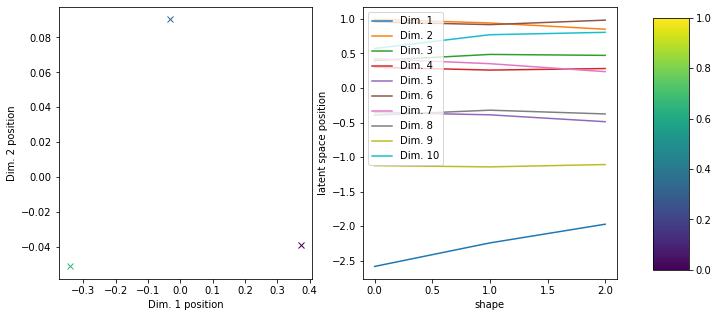
\includegraphics[width=\textwidth]{images/latent_space_traversals/vae_5000_dsprites_latent_space_values_shape.png}
        \caption{Traversal of the reduced latent space for different shapes.}
    \end{subfigure}
    \begin{subfigure}{.48\textwidth}
% include second image
        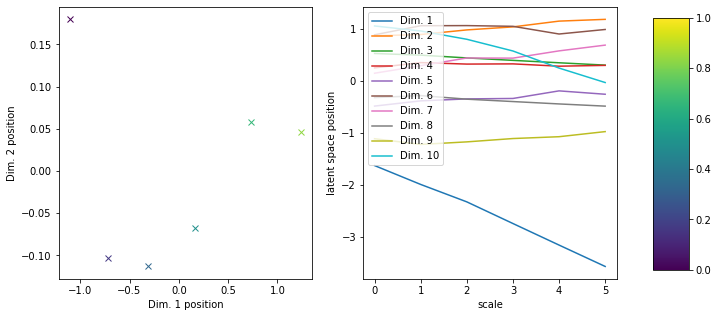
\includegraphics[width=\textwidth]{images/latent_space_traversals/vae_5000_dsprites_latent_space_values_scale.png}
        \caption{Traversal of the reduced latent space for different scales.}
    \end{subfigure}
    \begin{subfigure}{.48\textwidth}
% include second image
        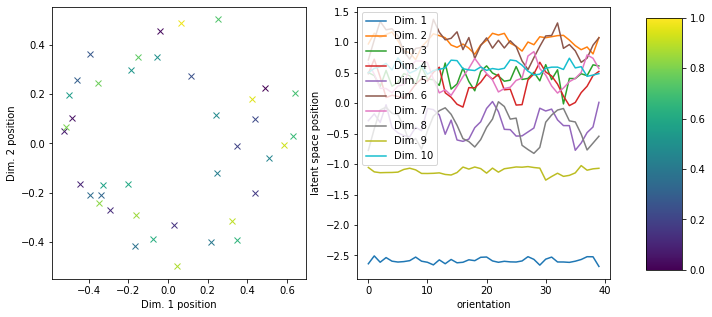
\includegraphics[width=\textwidth]{images/latent_space_traversals/vae_5000_dsprites_latent_space_values_orientation.png}
        \caption{Traversal of the reduced latent space for different orientations.}
    \end{subfigure}
    \caption[5,000-VAE - Latent Space Values]{Latent space of 5,000-\ac{VAE}. Different values correspond to different values for the respective factor of variation. For orientation and scale, the position is fixed to 0.0 in both directions, shape is fixed to \textit{Square}. For $x$-and $y$-postition, the other position is fixed to 1.0 and shape is fixed to \textit{Square}.}
    \label{fig:vae_dsprite_5000_latent_space_position}
\end{figure}

\begin{figure}[H]
    \centering
    \begin{subfigure}{.48\textwidth}
% include second image
        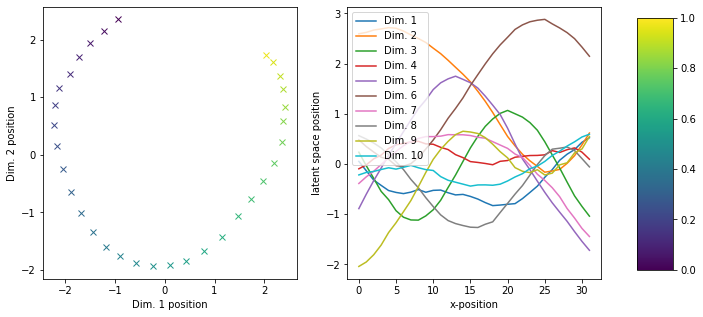
\includegraphics[width=\textwidth]{images/latent_space_traversals/vae_3750_dsprites_latent_space_values_x_position.png}
        \caption{Traversal of the reduced latent space for different $x$-positions.}
    \end{subfigure}
    \begin{subfigure}{.48\textwidth}
% include second image
        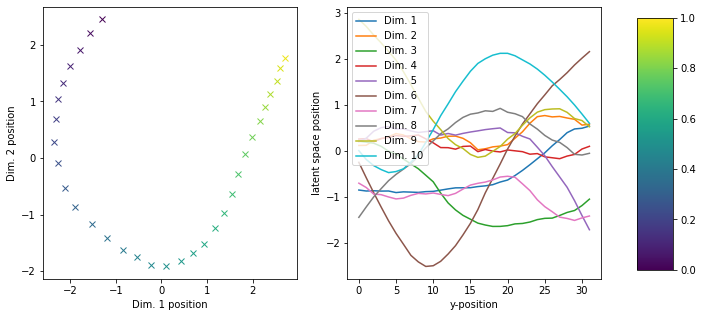
\includegraphics[width=\textwidth]{images/latent_space_traversals/vae_3750_dsprites_latent_space_values_y_position.png}
        \caption{Traversal of the reduced latent space for different $y$-positions.}
    \end{subfigure}
    \begin{subfigure}{.48\textwidth}
% include second image
        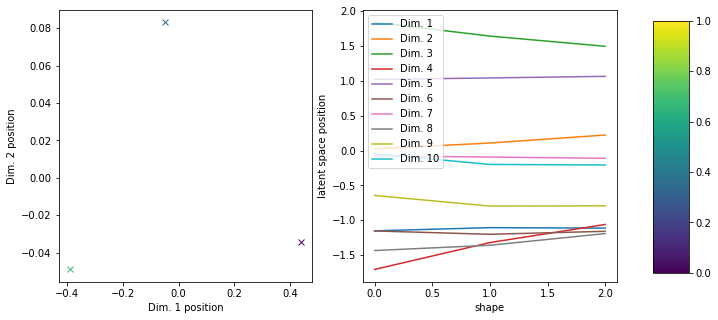
\includegraphics[width=\textwidth]{images/latent_space_traversals/vae_3750_dsprites_latent_space_values_shape.png}
        \caption{Traversal of the reduced latent space for different shapes.}
    \end{subfigure}
    \begin{subfigure}{.48\textwidth}
% include second image
        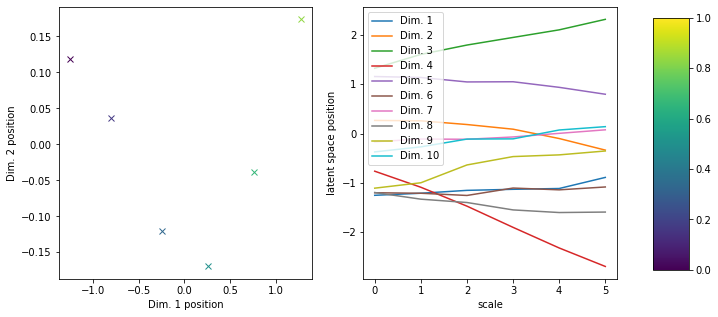
\includegraphics[width=\textwidth]{images/latent_space_traversals/vae_3750_dsprites_latent_space_values_scale.png}
        \caption{Traversal of the reduced latent space for different scales.}
    \end{subfigure}
    \begin{subfigure}{.48\textwidth}
% include second image
        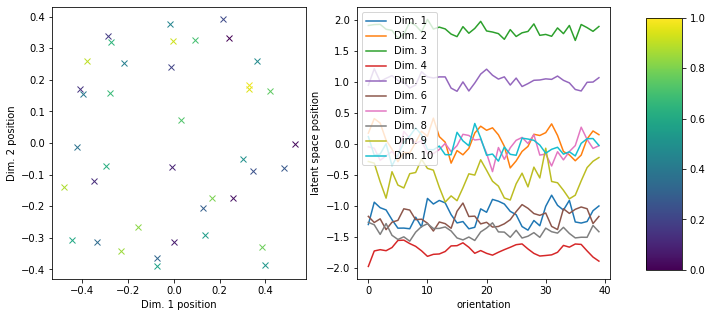
\includegraphics[width=\textwidth]{images/latent_space_traversals/vae_3750_dsprites_latent_space_values_orientation.png}
        \caption{Traversal of the reduced latent space for different orientations.}
    \end{subfigure}
    \caption[3,750-VAE - Latent Space Values]{Latent space of 3,750-\ac{VAE}. Different values correspond to different values for the respective factor of variation. For orientation and scale, the position is fixed to 0.0 in both directions, shape is fixed to \textit{Square}. For $x$-and $y$-postition, the other position is fixed to 1.0 and shape is fixed to \textit{Square}.}
    \label{fig:vae_dsprite_3750_latent_space_position}
\end{figure}

\begin{figure}
    \centering
    \begin{subfigure}{.48\textwidth}
        \centering
        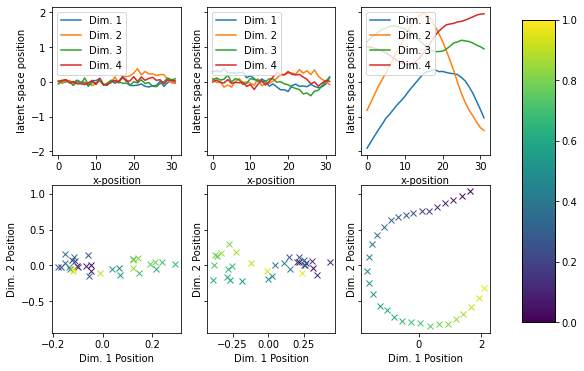
\includegraphics[width=\textwidth]{images/latent_space_traversals/vlae_gan_dsprites_left_latent_space_values.png}
        \caption{Varying $x$-position}
    \end{subfigure}
    \hfill
    \begin{subfigure}{.48\textwidth}
        \centering
        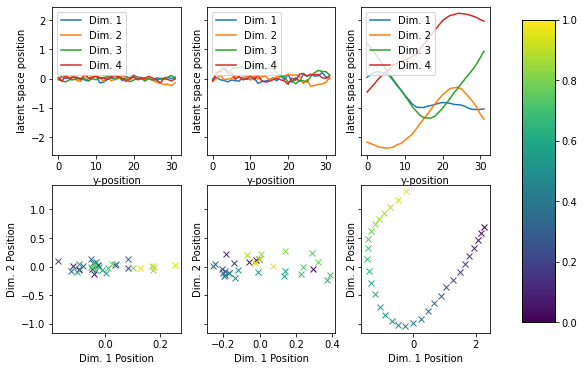
\includegraphics[width=\textwidth]{images/latent_space_traversals/vlae_gan_dsprites_bottom_latent_space_values.png}
        \caption{Varying $y$-position}
    \end{subfigure}
    \vfill
    \begin{subfigure}{.48\textwidth}
        \centering
        \includegraphics[width=\textwidth]{images/latent_space_traversals/vlae_gan_dsprites_orientation_latent_space_values.png}
        \caption{Varying orientation}
    \end{subfigure}
    \hfill
    \begin{subfigure}{.48\textwidth}
        \centering
        \includegraphics[width=\textwidth]{images/latent_space_traversals/vlae_gan_dsprites_scale_latent_space_values.png}
        \caption{Varying scale}
    \end{subfigure}
    \vfill
    \begin{subfigure}{.48\textwidth}
        \centering
        \includegraphics[width=\textwidth]{images/latent_space_traversals/vlae_gan_dsprites_shape_latent_space_values.png}
        \caption{Varying shape}
    \end{subfigure}
    \caption[dSprites-VLAE-GAN: Latent Space Values]{Values of different dimensions and layers in the dSprites-\ac{VLAE}-\ac{GAN} latent space for different factor of variation values (first row in each subplot), and position in a \ac{PCA}-reduced latent space (second row in each subplot). The left column corresponds to the first embedding layer, the right one to the third. \ac{PCA} was performed separately for each factor of variation and latent space layer. Different values correspond to different values for the respective factor of variation. For orientation and scale, the position is fixed to 0.0 in both directions, shape is fixed to \textit{Square}. For $x$-and $y$-postition, the other position is fixed to 1.0 and shape is fixed to \textit{Square}.}
    \label{fig:vlae_gan_dsprites_latent_space_values}
\end{figure}